\documentclass[sigconf,nonacm]{acmart}

% Packages
\usepackage{graphicx}
\usepackage{algorithm}
\usepackage{algpseudocode}
\usepackage{booktabs}
\usepackage{listings}
\usepackage{xcolor}
\let\Bbbk\relax
\usepackage{amsmath,amssymb,amsfonts}
\usepackage{hyperref}
\usepackage{tikz}
\usetikzlibrary{trees, positioning}

% ACM template cleanup
\settopmatter{printacmref=false}  % Remove ACM reference block
\renewcommand\footnotetextcopyrightpermission[1]{} % Remove footnote
\pagestyle{plain} % Only page numbers

% Listings style
\lstset{
  basicstyle=\footnotesize\ttfamily,
  breaklines=true,
  frame=single,
  backgroundcolor=\color{gray!5},
  keywordstyle=\color{blue}\bfseries,
  commentstyle=\color{green!50!black},
  numberstyle=\tiny,
  numbers=left,
  numbersep=6pt
}



% --------------------------------------------------
% Title & Authors
% --------------------------------------------------
\title{Blunder Guard: Efficient Small Language Models for Heuristic-Guided Chess Commentary Generation}

\author{Seyed Ali Hosseininasab}
\affiliation{
  \institution{Shahid Beheshti University}
  \city{Tehran}
  \country{Iran}
}
\email{seyed123ali123@gmail.com}

\author{Farima Kafi}
\affiliation{
  \institution{Shahid Beheshti University}
  \city{Tehran}
  \country{Iran}
}

\authornote{Instructor: Maryam Tahmasbi}

% --------------------------------------------------
\begin{document}

\begin{abstract}
We present \textbf{Blunder Guard}, a locally deployable system for generating pedagogical chess commentary by integrating a domain-adapted Small Language Model (SLM) with classical engine evaluation. A 1.7B-parameter Qwen3 model is fine-tuned on unstructured classical chess literature and guided at inference time by deterministic features, evaluations, and principal variations derived from Stockfish.

The training corpus comprises over 2.8M tokens extracted from canonical chess books using a parallelized PDF extraction pipeline. Positional features are computed from Stockfish evaluations and processed through a structured feature extractor before being fed into the SLM. The model is exported to GGUF for deployment with \texttt{llama.cpp}; the fine-tuned checkpoint evaluated in this report uses Q8\_0 quantization.

We evaluate seven candidate language models on 60 held-out position transitions divided equally among beginner, intermediate, and advanced strata. A local Gemma-family 12B model acts as a judge and scores correctness, instruction following, helpfulness, faithfulness, and fluency against curated references. The fine-tuned model is fluent but obtains only 2.49/10 overall, while the strongest tested hosted model obtains 7.31/10. The results show that local deployment is practical, but fluency alone does not establish chess-grounded correctness.

\end{abstract}

\keywords{Chess AI, Small Language Models, Explainable AI, Natural Language Generation}

\maketitle

\begin{figure}[htbp]
    \centering
    \resizebox{\columnwidth}{!}{%
        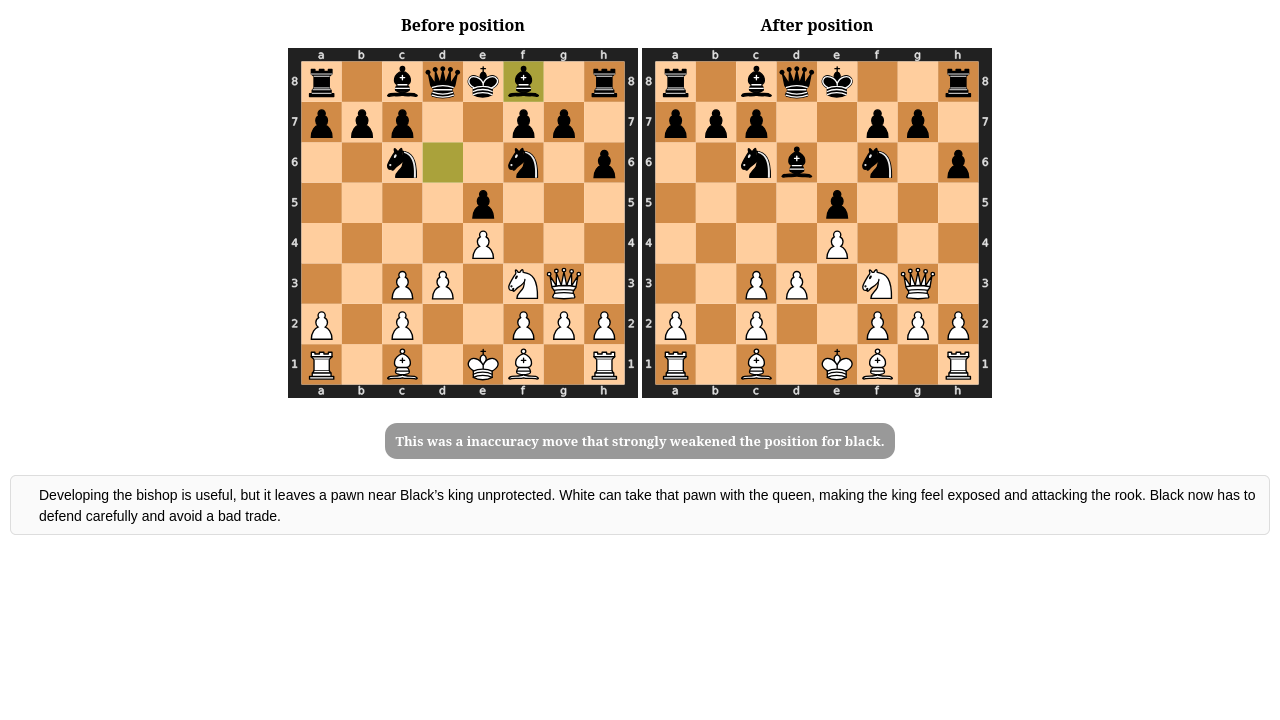
\includegraphics{prototype.jpg}%
    }
    \caption{Blunder Guard user interface showing interactive chessboard, real-time position analysis, and generated commentary for moves before and after evaluation.}
    \Description{A chessboard interface displaying the positions before and after a move together with generated explanatory commentary.}
    \label{fig:prototype}
\end{figure}


% ==================================================
\section{Introduction}
\label{sec:introduction}
% ==================================================

The confluence of superhuman chess engines and natural language generation presents a unique opportunity for chess education: explaining \emph{why} a position favors one side in terms accessible to human learners. Modern engines such as Stockfish~\cite{stockfish} and AlphaZero~\cite{alphazero} achieve tactical precision far beyond human masters, yet their output—centipawn evaluations and principal variations—remains opaque to intermediate players. Conversely, Large Language Models (LLMs) generate fluent explanations but frequently hallucinate tactical motifs and misevaluate positions, rendering them unreliable for serious instruction.

This work addresses the problem of \textbf{interpretable chess analysis}: generating commentary that is simultaneously (1) strategically accurate, grounded in objective engine evaluation; (2) pedagogically structured, following the conventions of classical chess literature; and (3) computationally efficient, enabling fully local deployment without cloud dependencies.

Existing approaches fall into two categories. Supervised methods~\cite{jhamtani2018chess} require large annotated datasets and lack scalability. LLM-based methods~\cite{kim2025ccc} achieve quality through scale but incur prohibitive costs and raise privacy concerns. Neither approach satisfies the needs of clubs, schools, or individual players seeking affordable, private coaching tools.

We propose a different paradigm: fine-tuning Small Language Models (SLMs) on unstructured chess literature while guiding generation with engine-verified heuristics. Canonical instructional texts encode reusable explanatory patterns without position-specific labels. By learning these patterns, an SLM can generalize to novel positions when guided by heuristic priorities derived from Stockfish, producing commentary that is both informative and pedagogically sound.


% ==================================================
\section{Related work}
\label{sec:related-work}
% ==================================================
The intersection of artificial intelligence and chess has long served as a testbed for exploring interpretable decision-making and natural language generation. While early approaches focused primarily on playing strength~\cite{deepblue,alphazero}, recent research has shifted toward making strong chess engines comprehensible to human players. This evolution reflects a broader trend in explainable AI: moving from black-box superhuman performance to systems that can articulate \textit{why} certain decisions are made~\cite{bjornsson2024chessxai}. In this context, chess commentary generation has emerged as a challenging benchmark, requiring models to balance strategic accuracy with pedagogical clarity. Unlike generic text generation, chess commentary demands domain knowledge, precise move grounding, and the ability to convey complex positional concepts in accessible language. The closest literature spans hand-crafted game features, learned neural-engine representations, symbolic-engine control signals, and explicit strategic concepts. Table~\ref{tab:related-comparison} summarizes the principal distinctions.

\begin{table*}[htbp]
\centering
\caption{Comparison with the closest chess explanation and commentary systems.}
\label{tab:related-comparison}
\begin{tabular}{@{}p{3.0cm}p{3.0cm}p{3.1cm}p{3.4cm}p{3.2cm}@{}}
\toprule
\textbf{Work} & \textbf{Chess grounding} & \textbf{Language supervision} & \textbf{Evaluation} & \textbf{Main distinction from Blunder Guard} \\
\midrule
Jhamtani et al.~\cite{jhamtani2018chess} & Hand-crafted move, threat, and engine-score features & 298K paired comments & Automatic metrics and human study & Supervised feature-aware generation \\
Zang et al.~\cite{zang2019automated} & Jointly trained neural chess engine & Paired comments by category & Automatic and human evaluation & Internal continuous engine representation \\
Lee et al.~\cite{lee2022improving} & Symbolic-engine control tags & Paired states and comments & Perplexity and human preference & Closest architecture; learned discrete control interface \\
Kim et al.~\cite{kim2025ccc} & Prioritized concepts from an expert model & Large-LLM generation & Human and GCC-Eval & Learned concept prioritization and LLM judge \\
Cui et al.~\cite{cui2026strategies} & Pruned branching engine strategy & Prompted LLM verbalization & Executability beyond the main line & Forward-looking strategy rather than post-hoc move explanation \\
Blunder Guard & Stockfish multi-PV plus board deltas & Unpaired chess books; constrained prompt & References scored by local Gemma-4-12B & Small local generator and deterministic, inspectable feature interface \\
\bottomrule
\end{tabular}
\end{table*}

\subsection{Bridging the Gap between Expert and Language Models}

Kim et al.~\cite{kim2025ccc} address a fundamental challenge in explainable artificial intelligence: bridging the gap between expert decision-making models and large language models (LLMs). While expert models such as modern chess engines achieve superhuman performance in complex decision-making tasks, their outputs are difficult for humans to interpret. In contrast, LLMs are capable of generating fluent and natural language explanations but often suffer from hallucinations and lack domain-specific reasoning capabilities. The authors study this problem in the context of chess commentary generation, which serves as a representative task for explaining complex decisions through natural language.

To overcome these limitations, the paper proposes a framework called \textit{Concept-guided Chess Commentary} (CCC). The key idea is to extract high-level chess concepts—such as king safety, passed pawns, mobility, and threats—from a neural chess expert model using concept-based explanation techniques. These concepts are represented as vectors learned via linear classifiers trained on positions labeled by a classical chess engine. For a given move, the framework prioritizes concepts by comparing their relevance before and after the move, identifying which concepts are most influential in explaining the decision.

The prioritized concepts are then provided as guidance to a large language model during commentary generation. This integration allows the LLM to focus on strategically important aspects of the position while avoiding incorrect or hallucinated explanations. As a result, the generated commentary is both linguistically fluent and strategically accurate.

In addition to commentary generation, the authors address the problem of evaluation. They introduce \textit{GPT-based Chess Commentary Evaluation} (GCC-Eval), a multi-dimensional evaluation framework that assesses commentary based on relevance, completeness, clarity, and fluency. Unlike traditional similarity-based metrics such as BLEU or ROUGE, GCC-Eval incorporates expert chess knowledge and shows a significantly higher correlation with human expert judgments.

Experimental results on a standard chess commentary dataset demonstrate that the proposed CCC framework outperforms existing baselines and even rivals human-generated commentary in terms of informativeness and linguistic quality. Overall, this work highlights the effectiveness of concept-based explanations as an interface between expert models and language models, and it provides a generalizable approach for interpretable decision explanation beyond the domain of chess.

\subsection{Engine-Conditioned Language Generation}

The closest architectural predecessor to Blunder Guard is Lee et al.~\cite{lee2022improving}. Their system combines a symbolic chess engine with a controllable language model. During training, it extracts control tags associated with properties such as move quality and the best continuation; during inference, a chess engine supplies those tags. Human judges preferred the engine-conditioned outputs to earlier baselines. Both systems therefore separate reliable chess calculation from natural-language realization. The important difference is the interface: Lee et al. learn from paired game-state/commentary data and condition generation with discrete control codes, whereas Blunder Guard fine-tunes on unpaired chess books and constructs a natural-language prompt from Stockfish multi-PV lines and deterministic before/after features. Their stronger supervised grounding helps explain why paired position-level data remains an important direction for our work.

Zang et al.~\cite{zang2019automated} integrate the expert more deeply. Their automated commentator jointly trains category-specific generation models with a neural chess engine that encodes boards, predicts moves, and represents likely future positions. They evaluate five commentary categories---description, move quality, context, comparison, and planning---using both automatic and human evaluation. This differs from Blunder Guard's modular use of an external Stockfish process: joint training may yield richer continuous board representations, while the modular approach permits a small generator, an independently replaceable engine, auditable features, and local deployment without training a chess-playing network.

\subsection{Learning to Generate Move-by-Move Chess Commentary}

Jhamtani et al.~\cite{jhamtani2018chess} study the task of automatically generating natural language commentary for individual moves in chess games. The authors frame this problem as a grounded natural language generation task, where the generated text must accurately reflect the game state, adhere to the rules of chess, and capture the strategic and pragmatic motivations behind a move. Chess commentary generation is particularly challenging due to the need for domain knowledge, the evolving nature of the game state, and the high variability in how humans describe the same move.

A major contribution of this work is the introduction of a large-scale chess commentary dataset collected from online chess forums. The dataset contains more than 298,000 move--commentary pairs spanning over 11,000 games, making it the first dataset of this scale for move-level chess commentary generation. An analysis of the data reveals substantial diversity in commentary styles, which the authors categorize into several types, including direct move descriptions, evaluations of move quality, comparisons with alternative moves, strategic planning explanations, contextual game-level information, and general comments. This diversity highlights the importance of content selection and pragmatic reasoning in the generation process.

To address these challenges, the authors propose a neural model called \textit{Game-Aware Commentary} (GAC). The model is trained end-to-end and incorporates multiple sources of domain-specific information extracted from the chess board state before and after a move. These features include move-related information (e.g., piece type and position), threat-related information (e.g., attacking and defending pieces), and score-based features obtained from a chess engine to estimate move quality. Feature representations are embedded in a shared continuous space, and a bidirectional LSTM encoder is used to model feature conjunctions. A selection mechanism is further employed to dynamically identify salient features during text generation, followed by an LSTM decoder that produces the commentary.

Experimental results show that the proposed GAC model outperforms several baselines, including template-based methods, nearest-neighbor approaches, and models that rely solely on raw board representations. Although automatic metrics such as BLEU yield relatively low scores due to the inherent variability of natural language commentary, human evaluation demonstrates that the generated commentaries are comparable to, and in some cases indistinguishable from, human-written commentary in terms of correctness and fluency. Overall, this work establishes a strong foundation for research on grounded and interpretable language generation in games and serves as a key reference for subsequent studies in chess commentary and explainable decision-making systems.

\subsection{From Move Commentary to Strategy Verbalization}

Cui et al.~\cite{cui2026strategies} formulate the newer task of \emph{chess strategy verbalization}. Instead of explaining only a move that has already been played, their pipeline extracts a pruned, branching strategy tree from an engine and asks a language model to communicate a forward-looking policy. Their evaluation tests whether a human or language-model player can execute the verbalized strategy, including responses outside the engine's main line. The study finds that concrete variations matter, that concept-only descriptions are limited, and that LLM-only evaluation has weaknesses. These observations are directly relevant to Blunder Guard: our current three-PV context is richer than a single evaluation but the generated response remains post-hoc and limited to two or three sentences. Extending evaluation from reference similarity to executable multi-branch plans would test whether commentary is practically useful rather than merely plausible.

Complementary interpretability work probes what chess engines know rather than generating commentary. P\'alsson and Bj\"ornsson~\cite{palsson2023concepts} apply probing methods to a superhuman chess agent and recover human-recognizable concepts from its neural representation. Bj\"ornsson's survey~\cite{bjornsson2024chessxai} places such work within the broader need for chess agents that explain the rationale behind their decisions. These studies support the premise that engine representations contain explainable strategic information, but they do not by themselves solve content selection or beginner-friendly language realization. Blunder Guard addresses this last interface explicitly through board-difference heuristics and constrained prompting.

% ==================================================
\section{Dataset Preparation}
\label{sec:dataset}
% ==================================================
In this section, we describe the construction of our training corpus and evaluation framework. Our approach diverges from conventional supervised learning: we employ a two-stage pipeline where (1) a Small Language Model (SLM) is first fine-tuned on pure chess literature without position-specific labels, and (2) a heuristic-enhanced evaluation system is subsequently applied to guide inference. This design choice prioritizes general strategic understanding over memorization of specific position-label pairs.


\subsection{Training Corpus Composition}
\label{subsec:corpus-comp}

The training dataset comprises curated classical chess literature representing diverse pedagogical approaches and historical periods. Unlike prior work that relies on annotated game databases with move-level labels~\cite{jhamtani2018chess}, our corpus consists of unstructured instructional text authored by renowned chess masters.

\subsubsection{Chess Literature Corpus}

We digitized five canonical chess instruction books:

\begin{itemize}
    \item \textit{The Game of Chess} by Siegbert Tarrasch (1935)~\cite{tarrasch1935game}: Foundational strategic principles and systematic piece development
    \item \textit{Zurich International Chess Tournament, 1953} by David Bronstein (1979)~\cite{bronstein1979zurich}: Deep annotations of candidate tournament games
    \item \textit{The Life and Games of Mikhail Tal} by Mikhail Tal (1997)~\cite{tal1997life}: Attacking patterns and dynamic piece play
    \item \textit{How to Reassess Your Chess} by Jeremy Silman (2010)~\cite{silman2010reassess}: Positional imbalances and modern strategic thinking
    \item \textit{Logical Chess: Move by Move} by Irving Chernev (1957)~\cite{chernev1957logical}: Pedagogical explanations for intermediate players
\end{itemize}

These texts span classical principles~\cite{tarrasch1935game}, modern imbalance theory~\cite{silman2010reassess}, tactical brilliance~\cite{tal1997life}, and instructional methodology~\cite{chernev1957logical}, providing comprehensive coverage of chess pedagogy.

\subsubsection{Text Extraction and Preprocessing}

Source materials existed in PDF format, necessitating robust extraction and cleaning. We developed a parallelized pipeline implemented in Python using \texttt{pypdf} for PDF parsing. Algorithm~\ref{alg:pdf-extraction} describes the extraction process.

\begin{algorithm}[htbp]
\caption{PDF Text Extraction Pipeline}
\label{alg:pdf-extraction}
\begin{algorithmic}[1]
\Require PDF directory $D_{pdf}$, Output directory $D_{txt}$
\Ensure Clean text files $T$
\State $F \gets \textsc{ListPDFs}(D_{pdf})$ \Comment{Enumerate PDF files}
\State $T \gets \emptyset$
\For{each file $f \in F$ \textbf{in parallel} using \texttt{ThreadPoolExecutor}}
    \State $text \gets \textsc{ExtractText}(f)$ \Comment{\texttt{PdfReader} page extraction}
    \State $text \gets \textsc{RemoveHyphenation}(text)$ \Comment{Join broken words}
    \State $text \gets \textsc{NormalizeWhitespace}(text)$ \Comment{Collapse multiple spaces/newlines}
    \If{$\textsc{Length}(text) > \theta_{min}$} \Comment{Filter empty/low-quality extractions}
        \State $t_{path} \gets \textsc{Save}(text, D_{txt}, \textsc{ChangeExtension}(f, .txt))$
        \State $T \gets T \cup \{t_{path}\}$
    \EndIf
\EndFor
\State \Return $T$
\end{algorithmic}
\end{algorithm}

The implementation handles critical PDF artifacts: line-break hyphenation (e.g., ``posi- tion'' $\rightarrow$ ``position'') and irregular whitespace from column layouts. Parallel processing utilizes all available CPU cores for efficient batch processing of the corpus. Total extracted text: approximately 2.8 million tokens after cleaning and deduplication.

\subsection{Heuristic Enhancement Module}
\label{subsec:heuristic}

Following model training, we employ a heuristic module to guide commentary generation during inference. This module bridges the gap between the model's general strategic knowledge and specific position evaluation, analogous to the concept extraction approach of Kim et al.~\cite{kim2025ccc} but implemented without requiring labeled training data.

Algorithm~\ref{alg:heuristic} describes the current Stockfish pipeline. For both the pre-move and post-move FEN, the engine searches to depth 17 with three principal variations. Scores and win probabilities are kept from White's point of view; the before/after delta is then sign-adjusted to the perspective of the player who made the move.

\begin{enumerate}
    \item Queries Stockfish~\cite{stockfish} for multi-PV evaluations, best moves, and forced-mate status.
    \item Infers the played move by replaying legal moves from the first FEN.
    \item Compares the two boards to detect concrete structural changes.
    \item Packages engine and heuristic evidence into one prompt-ready record.
\end{enumerate}

\begin{algorithm}[htbp]
\caption{Expert-Guided Move Evaluation with Structural Feature Extraction}
\label{alg:heuristic}
\small
\begin{algorithmic}[1]
\Require Position $FEN_{before}$, Position $FEN_{after}$
\Ensure Structured expert representation $S$

\State $E_{before},PV_{before},B \gets \textsc{MultiPV}(FEN_{before},3,17)$
\State $E_{after},PV_{after},B' \gets \textsc{MultiPV}(FEN_{after},3,17)$

\State $\Delta \gets \textsc{PerspectiveAdjustedDelta}(E_{before}, E_{after})$

\State $m \gets \textsc{InferPlayedMove}(FEN_{before}, FEN_{after})$

\State $F_{white} \gets \textsc{ExtractPositionFeatures}(FEN_{before}, FEN_{after}, \text{White})$
\State $F_{black} \gets \textsc{ExtractPositionFeatures}(FEN_{before}, FEN_{after}, \text{Black})$

\State $Q \gets \textsc{AssessMoveQuality}(\Delta, \textsc{MateStatus}(E_{after}))$

\State Construct structured record $S$ with:
\Statex \quad evaluations $(E_{before}, E_{after}, \Delta)$
\Statex \quad played move $m$, best moves $(B,B')$, and principal variations
\Statex \quad qualitative assessment $Q$
\Statex \quad feature deltas $(F_{white}, F_{black})$

\State \Return $S$
\end{algorithmic}
\end{algorithm}



The heuristic extracts a set of interpretable structural feature categories by comparing the board state before and after a move:
\begin{itemize}
    \item \textbf{Evaluation Shift}: Direction and magnitude of the engine-evaluated positional change, adjusted to the perspective of the player who made the move.
    \item \textbf{Material Safety}: Emergence of newly hanging or undefended pieces as a consequence of the move.
    \item \textbf{Pawn Structure}: Introduction of structural weaknesses such as doubled, isolated, or backward pawns.
    \item \textbf{King Safety}: Deterioration of defensive conditions, including loss of castling rights, increased attack pressure, or weakened pawn shields.
    \item \textbf{Positional Control}: Changes in control of e4, e5, d4, and d5, plus delayed development of bishops and knights.
    \item \textbf{Tactical Context}: Best moves before and after the transition, missed-opportunity text, and forced-mate information.
\end{itemize}

These features are derived through differential analysis of consecutive positions and do not rely on explicit tactical labels. The structured record contains the two FENs, Stockfish text, numeric evaluations, player-to-move fields, best moves, the played move, move-quality text, mate status, and feature dictionaries for both sides. This explicit interface is the main change from the earlier pipeline: candidate models receive both symbolic board changes and concrete multi-PV evidence rather than a single scalar engine score.

\subsection{Evaluation Data Construction}
\label{subsec:eval-data}

While our training corpus contains no position--commentary pairs, we construct a separate benchmark from the February 2013 Lichess standard-rated game database~\cite{lichesselite}. This benchmark is used only for assessment.

Games of at least 30 plies are grouped by the players' mean Elo: below 1200 for beginner, 1200--1799 for intermediate, and 1800 or above for advanced. Twenty manually selected transitions from each group form a balanced 60-row benchmark. For each transition, we record:

\begin{itemize}
    \item \textbf{FEN representations}: Before and after the move
    \item \textbf{Engine-grounded prompt}: Stockfish lines, feature changes, move classification, and mate information
    \item \textbf{Move context}: SAN notation, stable row identifier, and difficulty group
    \item \textbf{Reference explanation}: Curated learner-facing commentary used as judging ground truth
\end{itemize}

\begin{algorithm}[htbp]
\caption{Balanced Evaluation Benchmark Construction}
\label{alg:dataset-generation}
\begin{algorithmic}[1]
\Require Clustered PGN-derived games $G_c$, selected move indices $I_c$
\Ensure Balanced reference records $R$
\State $R \gets \emptyset$
\For{each difficulty $c \in \{beginner,intermediate,advanced\}$}
    \For{each selected index $i \in I_c$}
        \State $(FEN_b,FEN_a) \gets \textsc{ReplayToTransition}(G_c,i)$
        \State $S \gets \textsc{ExpertStructOutput}(FEN_b,FEN_a)$
        \State $p \gets \textsc{BuildPrompt}(S)$
        \State $r \gets \textsc{Record}(\textsc{StableId}(i),FEN_b,FEN_a,p,c)$
        \State $R \gets R \cup \{r\}$
    \EndFor
\EndFor \Comment{20 records per group, 60 total}
\State \Return $R$
\end{algorithmic}
\end{algorithm}

The evaluation records are stored as tab-separated values and aggregated from the three selected-move files. Candidate generation preserves \texttt{row\_id} and \texttt{type}, which permits strict one-to-one alignment with the reference. Model names are embedded in artifact filenames to prevent answer-model and judge-model metadata from drifting apart.

\begin{table}[htbp]
\centering
\caption{Evaluation Dataset Schema}
\label{tab:schema}
\resizebox{\columnwidth}{!}{%
\begin{tabular}{@{}llp{5.5cm}@{}}
\toprule
\textbf{Field} & \textbf{Type} & \textbf{Description} \\
\midrule
\texttt{before\_fen} & string & FEN before move \\
\texttt{after\_fen} & string & FEN after move \\
\texttt{move} & string & Move in SAN format (e.g., \texttt{Nf3}) \\
\texttt{prompt} & string & Engine-grounded candidate prompt \\
\texttt{analyse} & string & Curated reference commentary \\
\texttt{move type} & string & Engine-derived quality class \\
\texttt{type} & string & Beginner, intermediate, or advanced stratum \\
\bottomrule
\end{tabular}%
}
\end{table}

% ==================================================
\section{Methodology}
\label{sec:methodology}
% ==================================================
Blunder Guard is designed as a lightweight, deployable system for generating instructive chess commentary by combining classical engine evaluation with a Small Language Model (SLM). Rather than relying on large-scale end-to-end model training, the system emphasizes heuristic-guided inference, enabling strong explanatory performance while remaining feasible on consumer hardware. This section outlines the overall system architecture and data flow.

Figure~\ref{fig:structure} presents an abstract overview. The implemented API accepts two FEN strings, representing the board before and after a move. Stockfish analyzes both positions, the Python chess layer derives structural deltas, and the resulting evidence is serialized into a constrained beginner-oriented prompt. A quantized model served through \texttt{llama-server} generates the explanation, which Flask returns to the React client.


\begin{figure}[htbp]
    \centering
    \resizebox{\columnwidth}{!}{%
        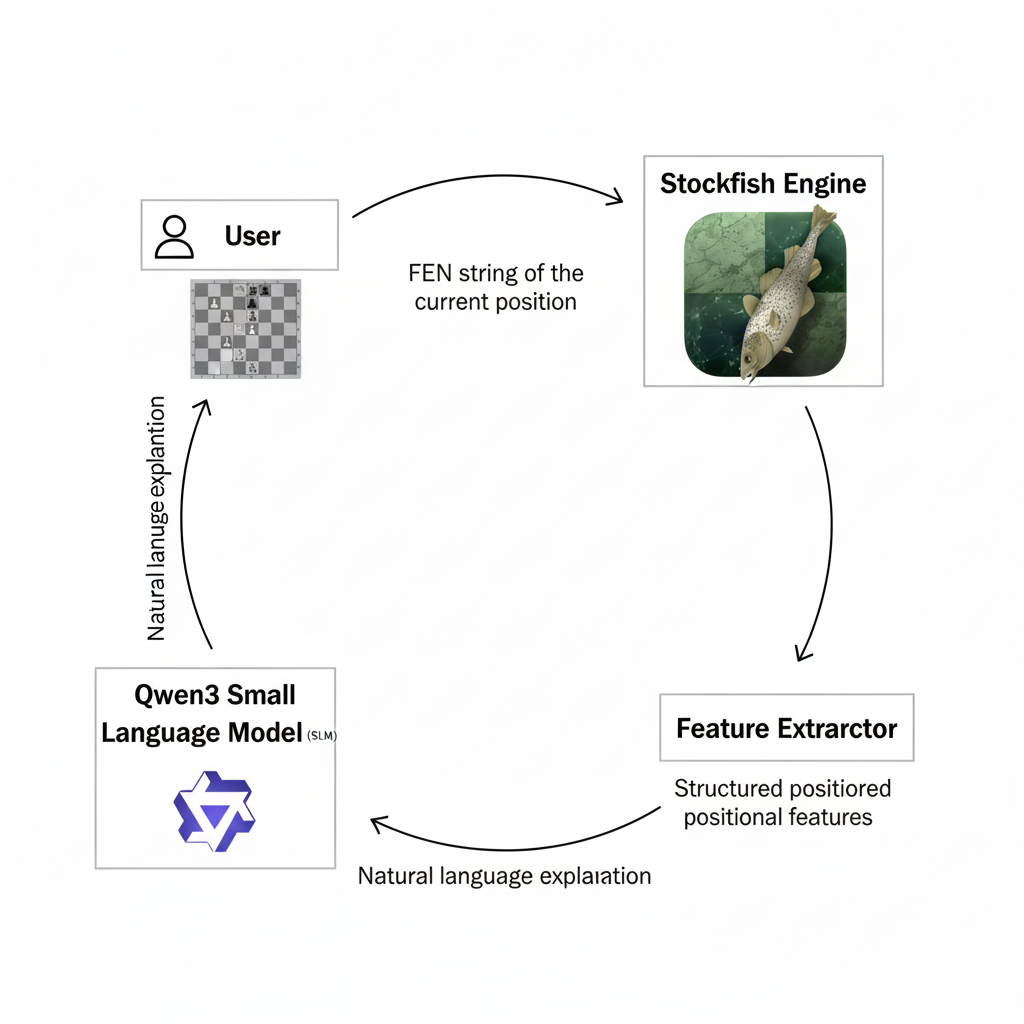
\includegraphics{structure_diagram.png}%
    }
    \caption{System architecture. The current implementation analyzes a position transition rather than a single isolated board.}
    \Description{Research pipeline connecting before-and-after chess positions, Stockfish analysis, structural feature extraction, and language-model commentary generation.}
    \label{fig:structure}
\end{figure}


\subsection{System Overview}

The Blunder Guard pipeline follows a modular, sequential design that integrates symbolic chess analysis with neural language generation. Given a chess position and a candidate move, the system produces a natural-language explanation assessing the move’s quality and underlying ideas.

The process begins with \textbf{engine-based analysis}. Stockfish is configured with 14 threads and a 2048 MB hash table. Each position is searched to depth 17 with three principal variations. The pipeline records the leading continuation, best move, centipawn score, transformed White win probability, and mate status.

Next, a deterministic \textbf{feature extraction module} compares the two legal board states. It detects newly hanging pieces, new doubled/isolated/backward pawns, degraded castling rights or pawn shields, increased king pressure, weakened control of central squares, and delayed minor-piece development. It also infers the played move and computes a player-perspective evaluation delta used to assign a qualitative move class.

Based on these features, the system constructs a \textbf{heuristic-guided prompt}. The prompt asks for two or three short sentences, prohibits engine terminology, numeric evaluations, and quoted lines, and supplies best moves and principal variations only as hidden reasoning context. This separates evidence acquisition from learner-facing verbalization.

Finally, the structured prompt is passed to a fine-tuned \textbf{Small Language Model}, which generates human-readable commentary explaining the move in an instructive style. The SLM operates purely at inference time, with no access to engine evaluations beyond what is encoded in the prompt.

This modular architecture decouples chess analysis, feature extraction, and language generation. It also permits the same 60 prompts to be sent either to a managed local GGUF server or to a hosted OpenAI-compatible endpoint, which is essential for the comparative evaluation in Section~\ref{sec:evaluation}.


\subsection{SLM Fine-Tuning}

To adapt the base language model to chess commentary, we perform targeted fine-tuning on our curated chess literature corpus. The fine-tuning procedure emphasizes efficient memory usage and stable training, enabling deployment on consumer-grade GPUs.

\subsubsection{Model Architecture}

The base model, \textbf{Qwen3-1.7B}, is a decoder-only transformer with 28 layers. Each layer contains multi-head attention and feed-forward submodules. Table~\ref{tab:model-arch} summarizes the key architectural components:

\begin{table*}[htbp]
\centering
\caption{Qwen3-1.7B Model Architecture Overview}
\label{tab:model-arch}
\begin{tabular}{@{}ll@{}}
\toprule
\textbf{Component} & \textbf{Details} \\
\midrule
Model type & Decoder-only Transformer (Qwen3ForCausalLM) \\
Embedding layer & Token embedding: 151,936 vocab size, hidden size 2048 \\
Number of layers & 28 (Qwen3DecoderLayer) \\
Attention & Qwen3Attention per layer: \\
& - Query projection: 2048$\rightarrow$2048 \\
& - Key projection: 2048$\rightarrow$1024 \\
& - Value projection: 2048$\rightarrow$1024 \\
& - Output projection: 2048$\rightarrow$2048 \\
& - Layer norms: q\_norm, k\_norm (RMSNorm, 128-dim) \\
Feed-forward network (MLP) & Gate: 2048$\rightarrow$6144 \\
& Up: 2048$\rightarrow$6144 \\
& Down: 6144$\rightarrow$2048 \\
& Activation: SiLU \\
Layer normalization & Input and post-attention RMSNorm (2048-dim) \\
Positional embedding & Rotary embedding \\
Language modeling head & Linear: 2048$\rightarrow$151,936 \\
\bottomrule
\end{tabular}
\end{table*}


Input sequences are tokenized and divided into 256-token chunks to optimize training efficiency while preserving context for long-form chess commentary.


\subsubsection{QLoRA Adaptation}

We employ \textbf{QLoRA}~\cite{dettmers2023qlora} (Quantized Low-Rank Adaptation) to efficiently adapt the base model using LoRA adapters. The LoRA configuration uses rank $r=16$ and scaling factor $\alpha=32$, applied to selected projection matrices within the attention layers (query and value projections). A small dropout of 0.05 and no bias terms are used to improve generalization and memory efficiency.

The training dataset is prepared as a \texttt{Dataset} object and fed to a \texttt{Trainer} instance from HuggingFace Transformers. Gradient accumulation is applied to simulate larger batch sizes, and mixed-precision training (FP16) reduces GPU memory usage. After training, the LoRA adapters are merged into the base model, producing a fully adapted model that can be saved and loaded for inference.

This fine-tuning approach balances computational efficiency with performance, enabling the SLM to produce fluent, chess-informed commentary without requiring full-parameter retraining.

\subsection{Quantization using \texttt{llama.cpp}}

To optimize the adapted Qwen3 model for local deployment on limited hardware, we employ \textbf{quantization} using the \texttt{llama.cpp} toolkit. Quantization reduces model size and memory footprint while maintaining acceptable accuracy for inference. In our workflow, the 16-bit floating-point model is converted to 8-bit using the following command:

\begin{lstlisting}[language=bash]
!llama.cpp/build/bin/llama-quantize \
    /kaggle/working/chess-fp16.gguf \
    /kaggle/working/chess-q8_0.gguf \
    q8_0
\end{lstlisting}

This produces a compressed model suitable for CPU and GPU inference, enabling efficient evaluation and integration into our Blunder Guard pipeline without sacrificing the quality of generated chess commentary.

\subsection{Feature Extraction and Prompting}

Our inference pipeline combines domain-specific chess knowledge from Stockfish with the generative capabilities of the fine-tuned LLM. The pipeline is designed to provide human-readable, pedagogical explanations of moves, suitable even for beginner players, while retaining the analytical rigor of engine evaluations.

\subsubsection{Positional Feature Extraction}

The first step combines Stockfish output with board-difference features computed using the \texttt{python}-\texttt{chess} library~\cite{pythonchess}. The current implementation captures:

\begin{itemize}
    \item \textbf{Central control}: Control over key central squares.
    \item \textbf{Material safety}: Newly attacked pieces that have no defender.
    \item \textbf{King safety}: Lost castling rights, added direct pressure, or a reduced pawn shield.
    \item \textbf{Pawn structure}: Newly doubled, isolated, or backward pawns.
    \item \textbf{Development and tactics}: Minor pieces remaining on their starting squares, best continuations, missed opportunities, and forced mate.
\end{itemize}

The numerical and line-based evidence is present in the prompt as context, but the output contract prevents the model from repeating it to a beginner. This distinction is important: the generator is exposed to engine evidence even though the final commentary should contain only its pedagogical interpretation.

\subsubsection{Inference Approaches}

We implement two complementary methods for generating move explanations:

\paragraph{Single Inference Method} In this approach, the LLM directly receives the positional features extracted from Stockfish and generates a natural language explanation in one step. This method is efficient and produces concise commentary, making it suitable for fast, real-time feedback or integration into a user interface where simplicity is preferred. The main steps are:

\begin{algorithm}[H]
\caption{Single Inference Method (Abstract)}
\begin{algorithmic}[1]
\Require Stockfish evaluation of current position
\Ensure Beginner-friendly move explanation
\State Extract position features from engine output
\State Construct a natural language prompt using these features
\State Feed the prompt into the LLM
\State Receive and return textual explanation
\end{algorithmic}
\end{algorithm}

\paragraph{Chain Inference Method} The chain inference method produces more nuanced explanations by performing multi-step reasoning. First, the LLM evaluates the positions \emph{before} and \emph{after} a move independently, generating structured descriptions for each. These intermediate outputs, together with Stockfish analysis, are then combined in a second prompt to produce a final explanation that clearly articulates why the move improved or weakened the position. This method allows the model to perform its own comparative reasoning in addition to leveraging engine insights, resulting in more detailed and instructive commentary. The workflow can be summarized as:

\begin{algorithm}[H]
\caption{Chain Inference Method (Abstract)}
\begin{algorithmic}[1]
\Require Stockfish analysis of \textbf{before} and \textbf{after} positions
\Ensure Detailed move explanation
\State Extract positional features for both before and after positions
\State Construct separate LLM prompts for each position
\State Feed prompts into LLM to obtain intermediate textual summaries
\State Compare before/after summaries with Stockfish evaluation
\State Construct a final LLM prompt incorporating all intermediate information
\State Feed final prompt into LLM
\State Receive and return the final textual explanation
\end{algorithmic}
\end{algorithm}

\subsubsection{Discussion and Use Cases}

The single inference method is ideal for scenarios requiring rapid evaluation or lightweight deployment, such as mobile apps or web interfaces. The chain inference method, although computationally heavier, is better suited for detailed post-game analysis, teaching tools, and generating insights that require reasoning over position changes. Together, these two approaches provide a flexible framework that balances speed, clarity, and analytical depth, ensuring the system can serve both casual players and serious learners.


\subsection{Deployment and Software Architecture}

The Blunder Guard system is implemented as a full-stack web application, combining a Python-based backend for chess analysis with a modern JavaScript frontend for interactive visualization. Unlike many academic or research-oriented projects, Blunder Guard is fully deployable, allowing users to run it locally or on any server, making it accessible across a wide range of devices from desktops to laptops and even mobile browsers. The backend handles model inference, Stockfish evaluation, and API endpoints, while the frontend provides a responsive interface for users to explore game commentary in real time.

\subsubsection{Backend}

The backend is implemented in the \texttt{app} directory using Python and Flask. It is responsible for:

\begin{itemize}
\item Serving API endpoints for LLM inference and Stockfish evaluation
\item Validating before/after FEN inputs supplied by the frontend
\item Integrating quantized Qwen3 LLM models using \texttt{llama.cpp} for efficient local inference on consumer-grade hardware
\item Returning a JSON object containing the generated commentary
\end{itemize}

\subsubsection{Frontend}

The frontend is implemented in the \texttt{frontend} directory using React and Bun. It provides:

\begin{itemize}
\item Interactive chessboard display with move highlighting
\item Commentary requests to the single-step and chain endpoints
\item Presentation of the generated move explanation
\item Adaptive design for desktop, tablet, and mobile devices, ensuring consistent user experience across platforms
\item A production build served directly by Flask
\end{itemize}

This architecture ensures smooth communication between the backend LLM inference engine and the frontend visualization, enabling an accessible, deployable, and fully operational chess coaching system that can be run on virtually any device without extensive setup.
The software interface is shown in Figure~\ref{fig:ui}.

\begin{figure}[htbp]
    \centering
    \resizebox{\columnwidth}{!}{%
        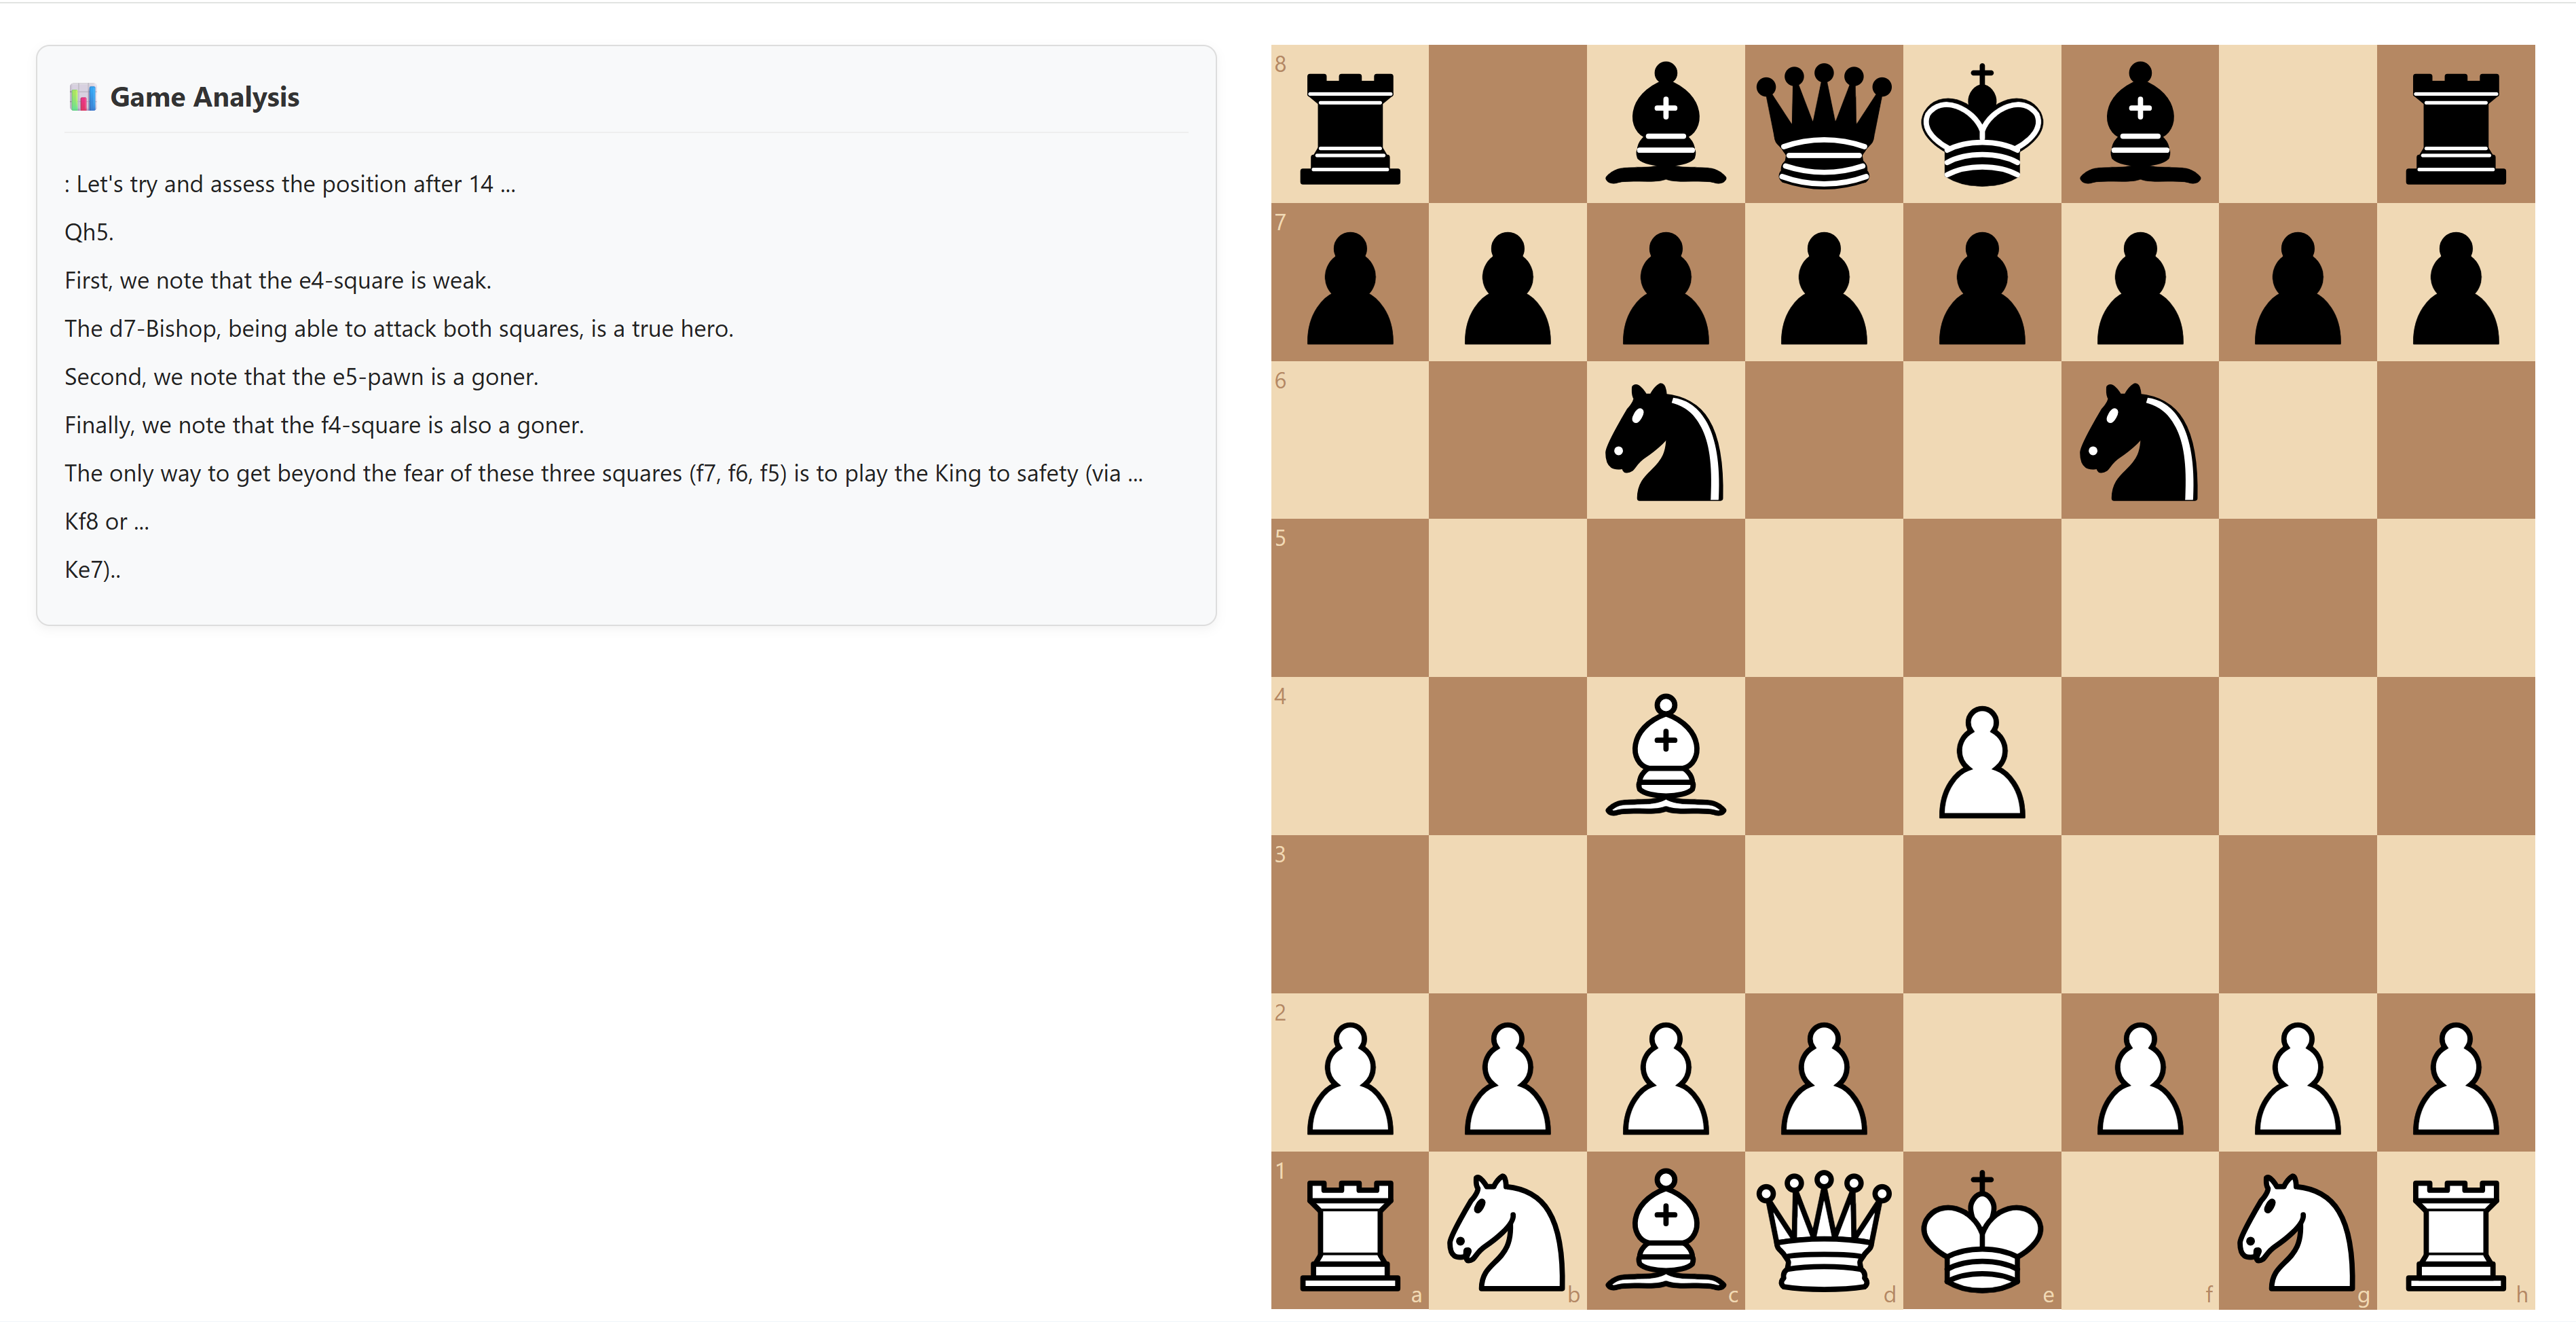
\includegraphics{software_screenshot.png}%
    }
    \caption{Blunder Guard user interface showing game analysis panel (left) and interactive chessboard (right).}
    \Description{The Blunder Guard analysis panel beside an interactive chessboard.}
    \label{fig:ui}
\end{figure}

% ==================================================
\section{Evaluation}
\label{sec:evaluation}
% ==================================================
Standard natural language generation metrics such as BLEU, ROUGE, and BERTScore are commonly used to evaluate text generation systems. However, these metrics are not suitable for our setting because \textbf{our training corpus contains no paired position--commentary data}. Unlike supervised approaches~\cite{jhamtani2018chess, kim2025ccc}, where models learn to reproduce human commentary for specific positions, Blunder Guard generates \emph{de novo} explanations based on general chess knowledge extracted from literature.

A generated explanation may be linguistically fluent yet strategically incorrect. For example, a commentary stating ``White gains a decisive advantage by activating the rook'' may read well but be objectively false if the position is evaluated as equal by Stockfish. Conversely, a factually correct explanation phrased in a non-canonical style may appear stylistically unusual while being practically more useful.

\subsection{Candidate Models and Protocol}

We evaluate seven answer models: the fine-tuned Qwen3 model (\texttt{chess-q8\_0}), Llama-3.2-3B-Instruct, Gemma-3-12B-Instruct, Gemini-3.5-Flash, GPT-5.5, Grok-4.3, and Qwen3.7-Plus. Each model receives the same 60 engine-grounded prompts. Local GGUF models are launched through a managed \texttt{llama-server}; hosted models are accessed through an OpenAI-compatible API. The answer-model identity is stored both in each row and in the output filename.

We then compare every candidate response with its aligned reference using a local \textbf{Gemma 4 12B judge}~\cite{gemma4}. This follows the LLM-as-a-judge paradigm~\cite{zheng2023judging}, adapted to reference-grounded chess evaluation. Reasoning is disabled, temperature is zero, and the judge is required to return schema-constrained JSON. It assigns independent integer scores from 0 to 10 for:

\begin{itemize}
    \item \textbf{Correctness}: Agreement with the central chess claims in the reference.
    \item \textbf{Instruction following}: Relevance as a learner-facing chess explanation.
    \item \textbf{Helpfulness}: Communication of the reference lesson, cause, or consequence.
    \item \textbf{Faithfulness}: Avoidance of claims unsupported by the reference.
    \item \textbf{Fluency}: Grammar and clarity, scored independently of factual accuracy.
\end{itemize}

The application calculates a weighted overall score:
\begin{equation}
O=0.35C+0.25F+0.20H+0.10I+0.10L,
\end{equation}
where $C$, $F$, $H$, $I$, and $L$ denote correctness, faithfulness, helpfulness, instruction following, and fluency. Correctness and faithfulness therefore account for 60\% of the final score. Candidate/reference rows are aligned by difficulty type and stable row ID. All 420 judgments parsed successfully; no Qwen-judge output is included in the reported results.

\subsection{Results}

Table~\ref{tab:judge-results} reports means over all 60 positions for each answer model. GPT-5.5 ranks first with 7.31 overall, followed by Qwen3.7-Plus (6.50), Gemini-3.5-Flash (6.46), and Grok-4.3 (5.44). The three local models score below 3.0. The fine-tuned \texttt{chess-q8\_0} model obtains 2.49, below the untuned Llama-3.2-3B (2.86) and Gemma-3-12B (2.95) baselines.

\begin{table*}[htbp]
\centering
\caption{Gemma-4-12B judge means over 60 positions per answer model (0--10).}
\label{tab:judge-results}
\begin{tabular}{@{}lrrrrrr@{}}
\toprule
\textbf{Answer model} & \textbf{Correct.} & \textbf{Instr.} & \textbf{Helpful} & \textbf{Faithful} & \textbf{Fluent} & \textbf{Overall} \\
\midrule
GPT-5.5 & 6.28 & 9.85 & 7.57 & 6.43 & 10.00 & \textbf{7.31} \\
Qwen3.7-Plus & 5.30 & 10.00 & 6.63 & 5.27 & 10.00 & 6.50 \\
Gemini-3.5-Flash & 5.15 & 9.97 & 6.70 & 5.27 & 10.00 & 6.46 \\
Grok-4.3 & 3.92 & 9.90 & 5.27 & 4.08 & 10.00 & 5.44 \\
Gemma-3-12B-Instruct Q4 & 0.88 & 10.00 & 2.03 & 0.92 & 10.00 & 2.95 \\
Llama-3.2-3B-Instruct Q4 & 0.83 & 9.40 & 1.95 & 0.93 & 10.00 & 2.86 \\
Fine-tuned chess Q8 & 0.83 & 7.22 & 1.82 & 0.88 & 8.97 & 2.49 \\
\bottomrule
\end{tabular}
\end{table*}

Figure~\ref{fig:metric-means} makes the separation between surface quality and grounding visible. Most models receive near-perfect fluency and instruction-following scores, while correctness and faithfulness determine the ranking. Figure~\ref{fig:category-results} shows that advanced positions are generally harder: for example, Gemini falls from 7.10 on beginner positions to 5.19 on advanced positions, and GPT-5.5 falls from 7.36 to 6.72. Qwen3.7-Plus is comparatively stable across the three groups.

\begin{figure*}[htbp]
    \centering
    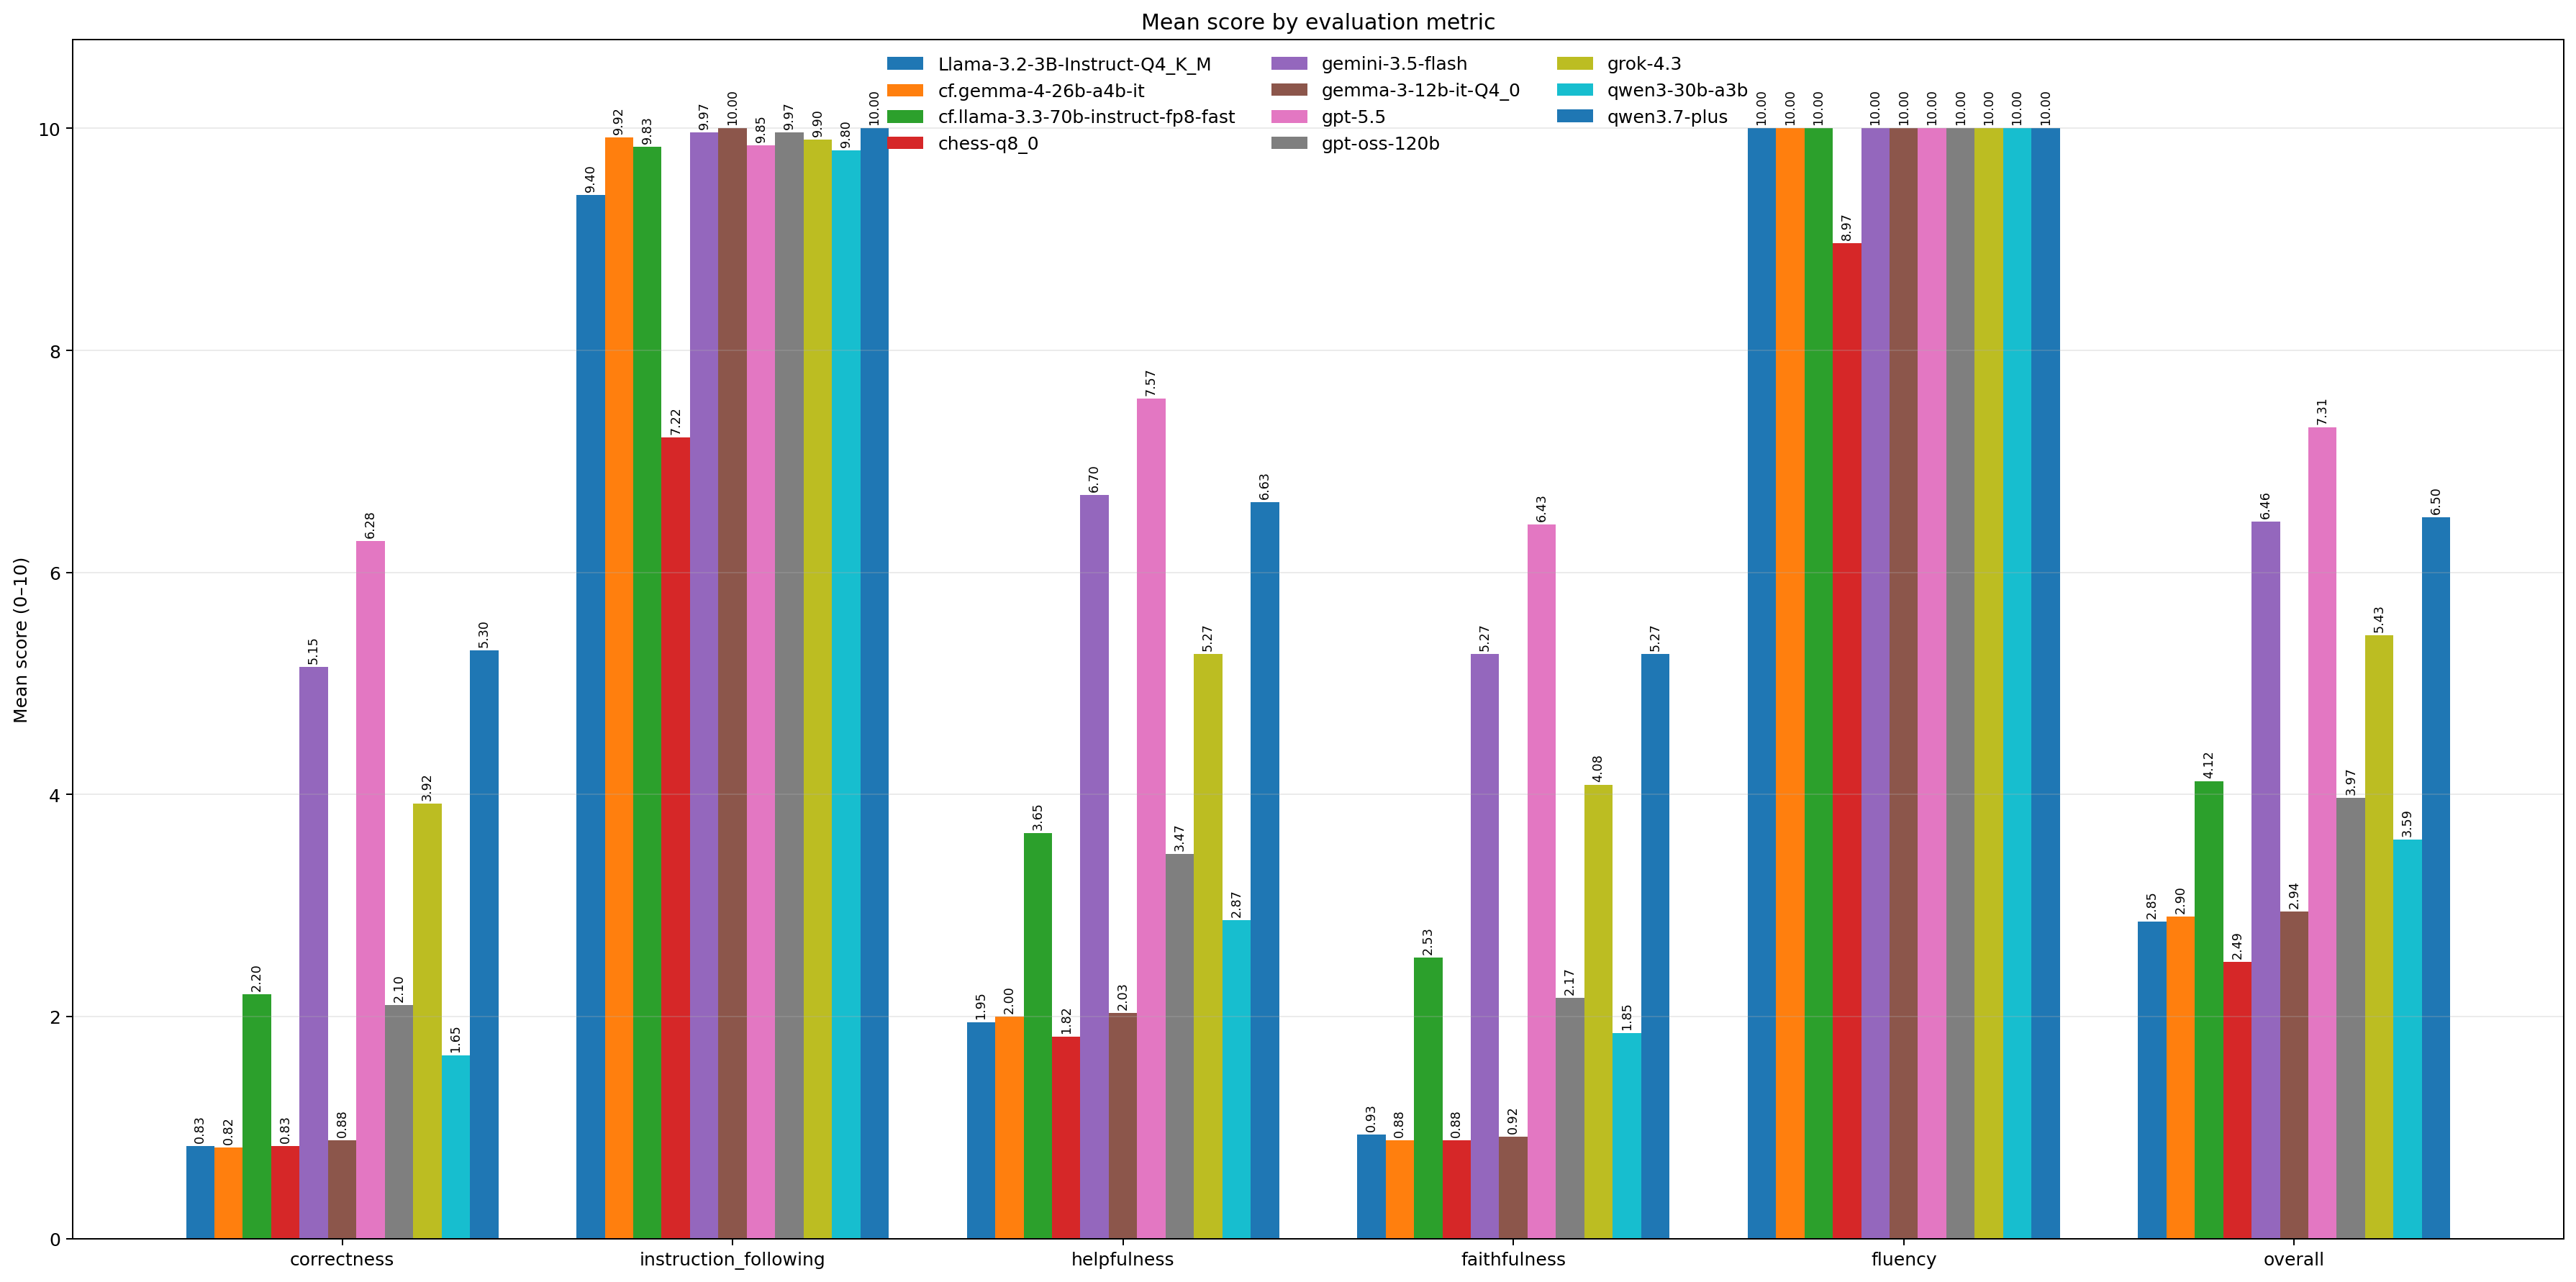
\includegraphics[width=\textwidth]{gemma4_judge_plots/01_metric_means.png}
    \caption{Mean metric scores for seven answer models, evaluated only by the Gemma-4-12B judge.}
    \Description{Grouped bars comparing correctness, instruction following, helpfulness, faithfulness, fluency, and overall scores for seven answer models.}
    \label{fig:metric-means}
\end{figure*}

\begin{figure}[htbp]
    \centering
    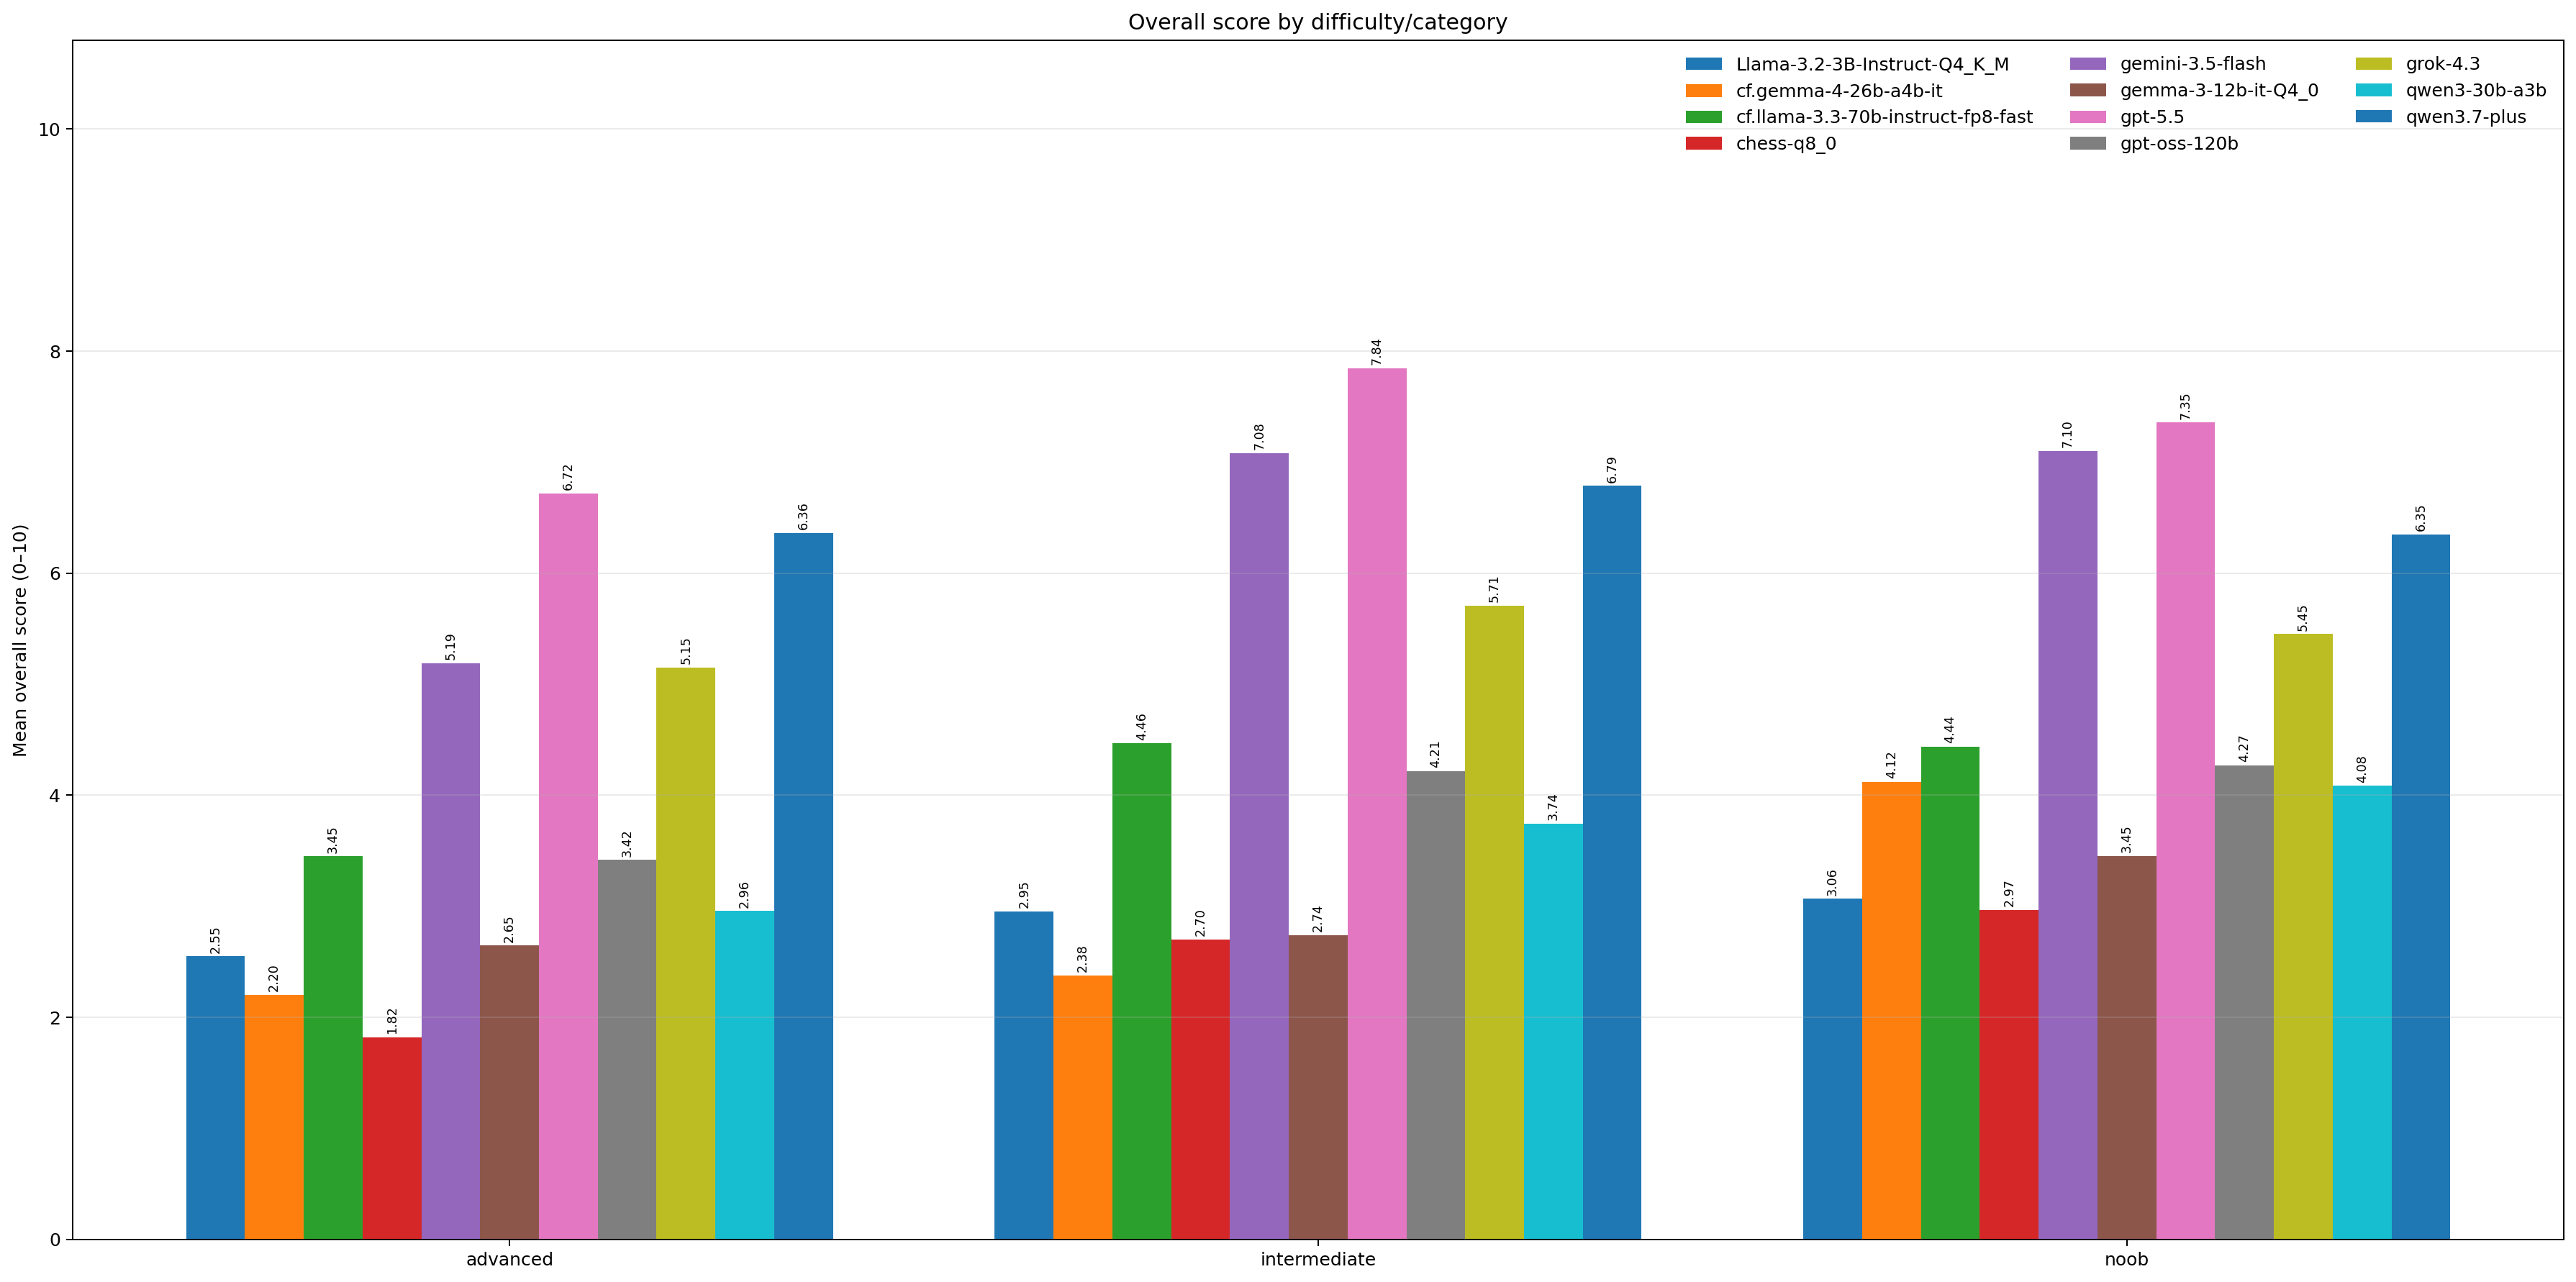
\includegraphics[width=\columnwidth]{gemma4_judge_plots/02_category_comparison.png}
    \caption{Mean weighted overall score by benchmark difficulty. Each model has 20 positions per group.}
    \Description{Grouped bars comparing the overall model scores on advanced, beginner, and intermediate chess positions.}
    \label{fig:category-results}
\end{figure}

These results do not support the earlier qualitative claim that the fine-tuned small model is reliably strategically accurate. They instead show that its text can look plausible while disagreeing with the reference lesson or introducing unsupported chess claims. Fine-tuning on unpaired books appears to improve domain style less reliably than explicit position-grounded supervision would improve factual alignment.

% ==================================================
\section{Discussion}
\label{sec:discussion}
% ==================================================
Blunder Guard demonstrates a complete lightweight pipeline for combining classical engine evidence with language generation, but the quantitative evaluation also identifies a clear quality limit. The fine-tuned model follows the intended local-deployment design, yet it does not reliably translate the supplied evidence into reference-aligned chess explanations.

\subsection{Strengths of the Approach}

Our methodology has several notable advantages:

\begin{itemize}
    \item \textbf{Efficiency and Deployability:} The system can run on consumer-grade hardware thanks to LoRA fine-tuning and quantization with \texttt{llama.cpp}, making it more accessible than larger, end-to-end models.
    \item \textbf{Inspectable grounding:} Stockfish lines, scores, best moves, mate status, and deterministic board features are separated from generation and can be audited independently.
    \item \textbf{Flexibility:} The dual inference methods—single-step and chain inference—allow trade-offs between speed and depth of explanation.
\end{itemize}

\subsection{Limitations}

Despite these strengths, several limitations should be acknowledged:

\begin{itemize}
    \item \textbf{Judge dependence:} Scores come from one local Gemma-4-12B judge. Although deterministic prompts, strict JSON, references, and independent metrics improve reproducibility, LLM judgments can contain systematic bias and should be calibrated against rated human evaluators.
    \item \textbf{Reference dependence:} Each candidate is compared with one curated explanation. A different but valid strategic explanation can receive too little credit, while errors in a reference propagate into every candidate score.
    \item \textbf{Small benchmark:} The benchmark contains only 60 positions (20 per group), so small differences between similarly ranked models should not be treated as definitive.
    \item \textbf{Weak fine-tuned result:} The fine-tuned model's 2.49 overall score and sub-1.0 correctness/faithfulness means show that unpaired book fine-tuning plus prompt grounding is insufficient for reliable commentary.
    \item \textbf{Limited Contextual Depth:} The model operates primarily on immediate positional features and may miss long-term strategic plans that extend beyond the analyzed move.
    \item \textbf{Chess Knowledge Dependency:} The system relies on Stockfish for objective evaluation. In positions where engine assessments are ambiguous or non-intuitive, the commentary may lack subtlety appreciated by human players.
\end{itemize}

\subsection{Future Directions}

There are several avenues to improve and extend Blunder Guard:

\begin{itemize}
    \item \textbf{Supervised Data Integration:} Incorporating labeled position-commentary pairs could improve the model's ability to generate accurate and instructive commentary. Such datasets could be created either by expert annotators or by leveraging LLMs to generate synthetic training data.
    \item \textbf{Hardware Optimization:} Optimizing the model to run efficiently on NPUs, mobile devices, or local systems would enhance accessibility and real-time inference capabilities.
    \item \textbf{Expanded Knowledge Base:} Integrating additional chess literature and opening/middle/endgame manuals could improve the breadth and depth of the model’s strategic understanding.
    \item \textbf{Robust Evaluation on Seen vs. Unseen Positions:} Splitting chess positions from the training books and evaluating on unseen positions would allow a more systematic assessment of the model’s generalization capabilities.
    \item \textbf{Sequence-Level Analysis:} Extending the chain inference method to multi-move sequences could enable the generation of commentary for positional trends and long-term planning.
    \item \textbf{Human calibration of the judge:} A blinded expert study should measure correlation between Gemma-4-12B scores and rated-player judgments, including inter-annotator agreement.
    \item \textbf{Ablation studies:} Stockfish lines, structural features, book fine-tuning, and chain prompting should be removed one at a time to determine which components improve correctness rather than only fluency.
\end{itemize}

Overall, the engineering architecture is promising for accessible chess explanation, but the present small-model checkpoint should be treated as a prototype rather than a reliable coach. The evaluation indicates that future work must prioritize factual grounding and position-specific supervision over stylistic fluency.


% ==================================================
\section{Conclusion}
\label{sec:conclusion}
% ==================================================

We presented \textbf{Blunder Guard}, a lightweight, deployable system for chess commentary that combines depth-17 multi-PV Stockfish analysis, deterministic board-difference features, constrained prompting, and quantized local inference. The application and evaluation tools run through OpenAI-compatible interfaces, allowing local and hosted answer models to be compared under one artifact-tracked pipeline.

On 60 curated positions, the Gemma-4-12B judge ranks GPT-5.5 highest at 7.31/10, while the fine-tuned local chess model scores 2.49/10. Its relatively high fluency does not compensate for low correctness and faithfulness. The principal conclusion is therefore methodological rather than a claim of solved commentary generation: engine grounding is necessary, but the current prompt and unpaired book fine-tuning do not ensure that a small model uses that evidence correctly. Position-grounded training, larger benchmarks, ablations, and human calibration are required before deployment as a dependable instructional system.


\begin{acks}
This work was supported by publicly available chess literature, the Stockfish engine, Qwen3 and open-source software such as \texttt{llama.cpp}, which enabled local inference and model quantization.
\end{acks}


% ==================================================
\bibliographystyle{ACM-Reference-Format}
\bibliography{references}

\end{document}
